\documentclass[9pt]{scrartcl}

\usepackage[utf8]{inputenc}
\usepackage[italian]{babel}

\pagestyle{empty}

\usepackage[default]{lato}

\usepackage{geometry}
\geometry{
  % a4paper,
  letterpaper,
  top=\dimexpr1.5in+0.5in\relax, % 0.5in from ribbon
  left=\dimexpr3.0in\relax, % 0.5in from ribbon
  right=0.5in,
  bottom=.5in,
  % showframe
}

\usepackage{csquotes}

\usepackage{parskip}
\linespread{1.2}

\usepackage{fontawesome}

\usepackage[hidelinks]{hyperref}
\urlstyle{sf}

%===[ TYPESETTING ]=============================================================

\usepackage{multicol}

\setlength{\multicolsep}{0pt}

\usepackage{enumitem}

\SetEnumitemKey{twocol}{
% itemsep=1\itemsep,
% parsep=1\parsep,
before=\vspace{\parskip}\raggedcolumns\begin{multicols}{2},
after=\end{multicols}}

\setlist[itemize]{nosep,wide,leftmargin=1em,labelwidth=1em,labelsep=0pt}









%===[ MACRO TRICKERY ]==========================================================

\usepackage{xparse}
% \usepackage{etoolbox}

\NewDocumentCommand{\Section}{m}{
\medskip
\begingroup
% \fontseries{l}
\large\scshape
\lsstyle
\hrulefill\quad
\MakeUppercase{#1}
\quad\hrulefill
\endgroup
}

\NewDocumentCommand{\Event}{mmm}
  {\smallskip{\bfseries#1}\hfill\emph{#2}\quad#3}

\NewDocumentCommand{\Rank}{mO{5}}{%
  \newcount\N
  \N=0
  $\loop\ifnum\N<#2
    \ifnum\N<#1\bullet\else\circ\fi
    \advance \N by 1
  \repeat$}

\NewDocumentCommand{\Ranked}{mmO{5}}{%
  \begingroup%
  \ifnum#2<2
    \fontseries{l}
  \else\ifnum\numexpr2*#2\relax<#3\else
    \fontseries{eb}
  \fi\fi\selectfont
  #1\endgroup\hfill\Rank{#2}[#3]\par}

\NewDocumentCommand{\Fa}{m}
  {\hbox to 1em{\hfill\resizebox{1em}{!}{\csname fa#1\endcsname}\hfill}}

\NewDocumentCommand{\SideSection}{m}
  {{\scshape\large#1\quad\hrulefill}\par\smallskip}

%===[ DRAWING TOOLS ]===========================================================

\usepackage{xcolor}
\usepackage{eso-pic}
\usepackage{tikz}
\usetikzlibrary{positioning}
\usetikzlibrary{calc}

\def\q{*0.25in}


\AddToShipoutPictureBG{%
  \begin{tikzpicture}[remember picture,overlay]
    \fill
      [violet!15!white]
      ($(current page.north west)+(0,-1\q)$)
      rectangle
      ($(current page.north east)+(0,-7\q)$);
    \fill
      [violet!50!black]
      ($(current page.north west)+(1\q,0)$)
      rectangle
      ($(current page.south west)+(11\q,0)$);
    \node [
        anchor=west,
        % draw,
        font=\fontseries{l}\selectfont\lsstyle,
        inner sep=0,
        text width=4.25in,
      ] at (14\q,40\q)
      {\resizebox{4.25in}{!}{\MakeUppercase{Paolo \ Brasolin}}};
    \begin{scope}[shift={(6\q,39\q)}]
      \clip circle (4\q);
      \fill [white] circle (5\q);
      \node[shift={(.04in,-.075in)},scale=1.1]{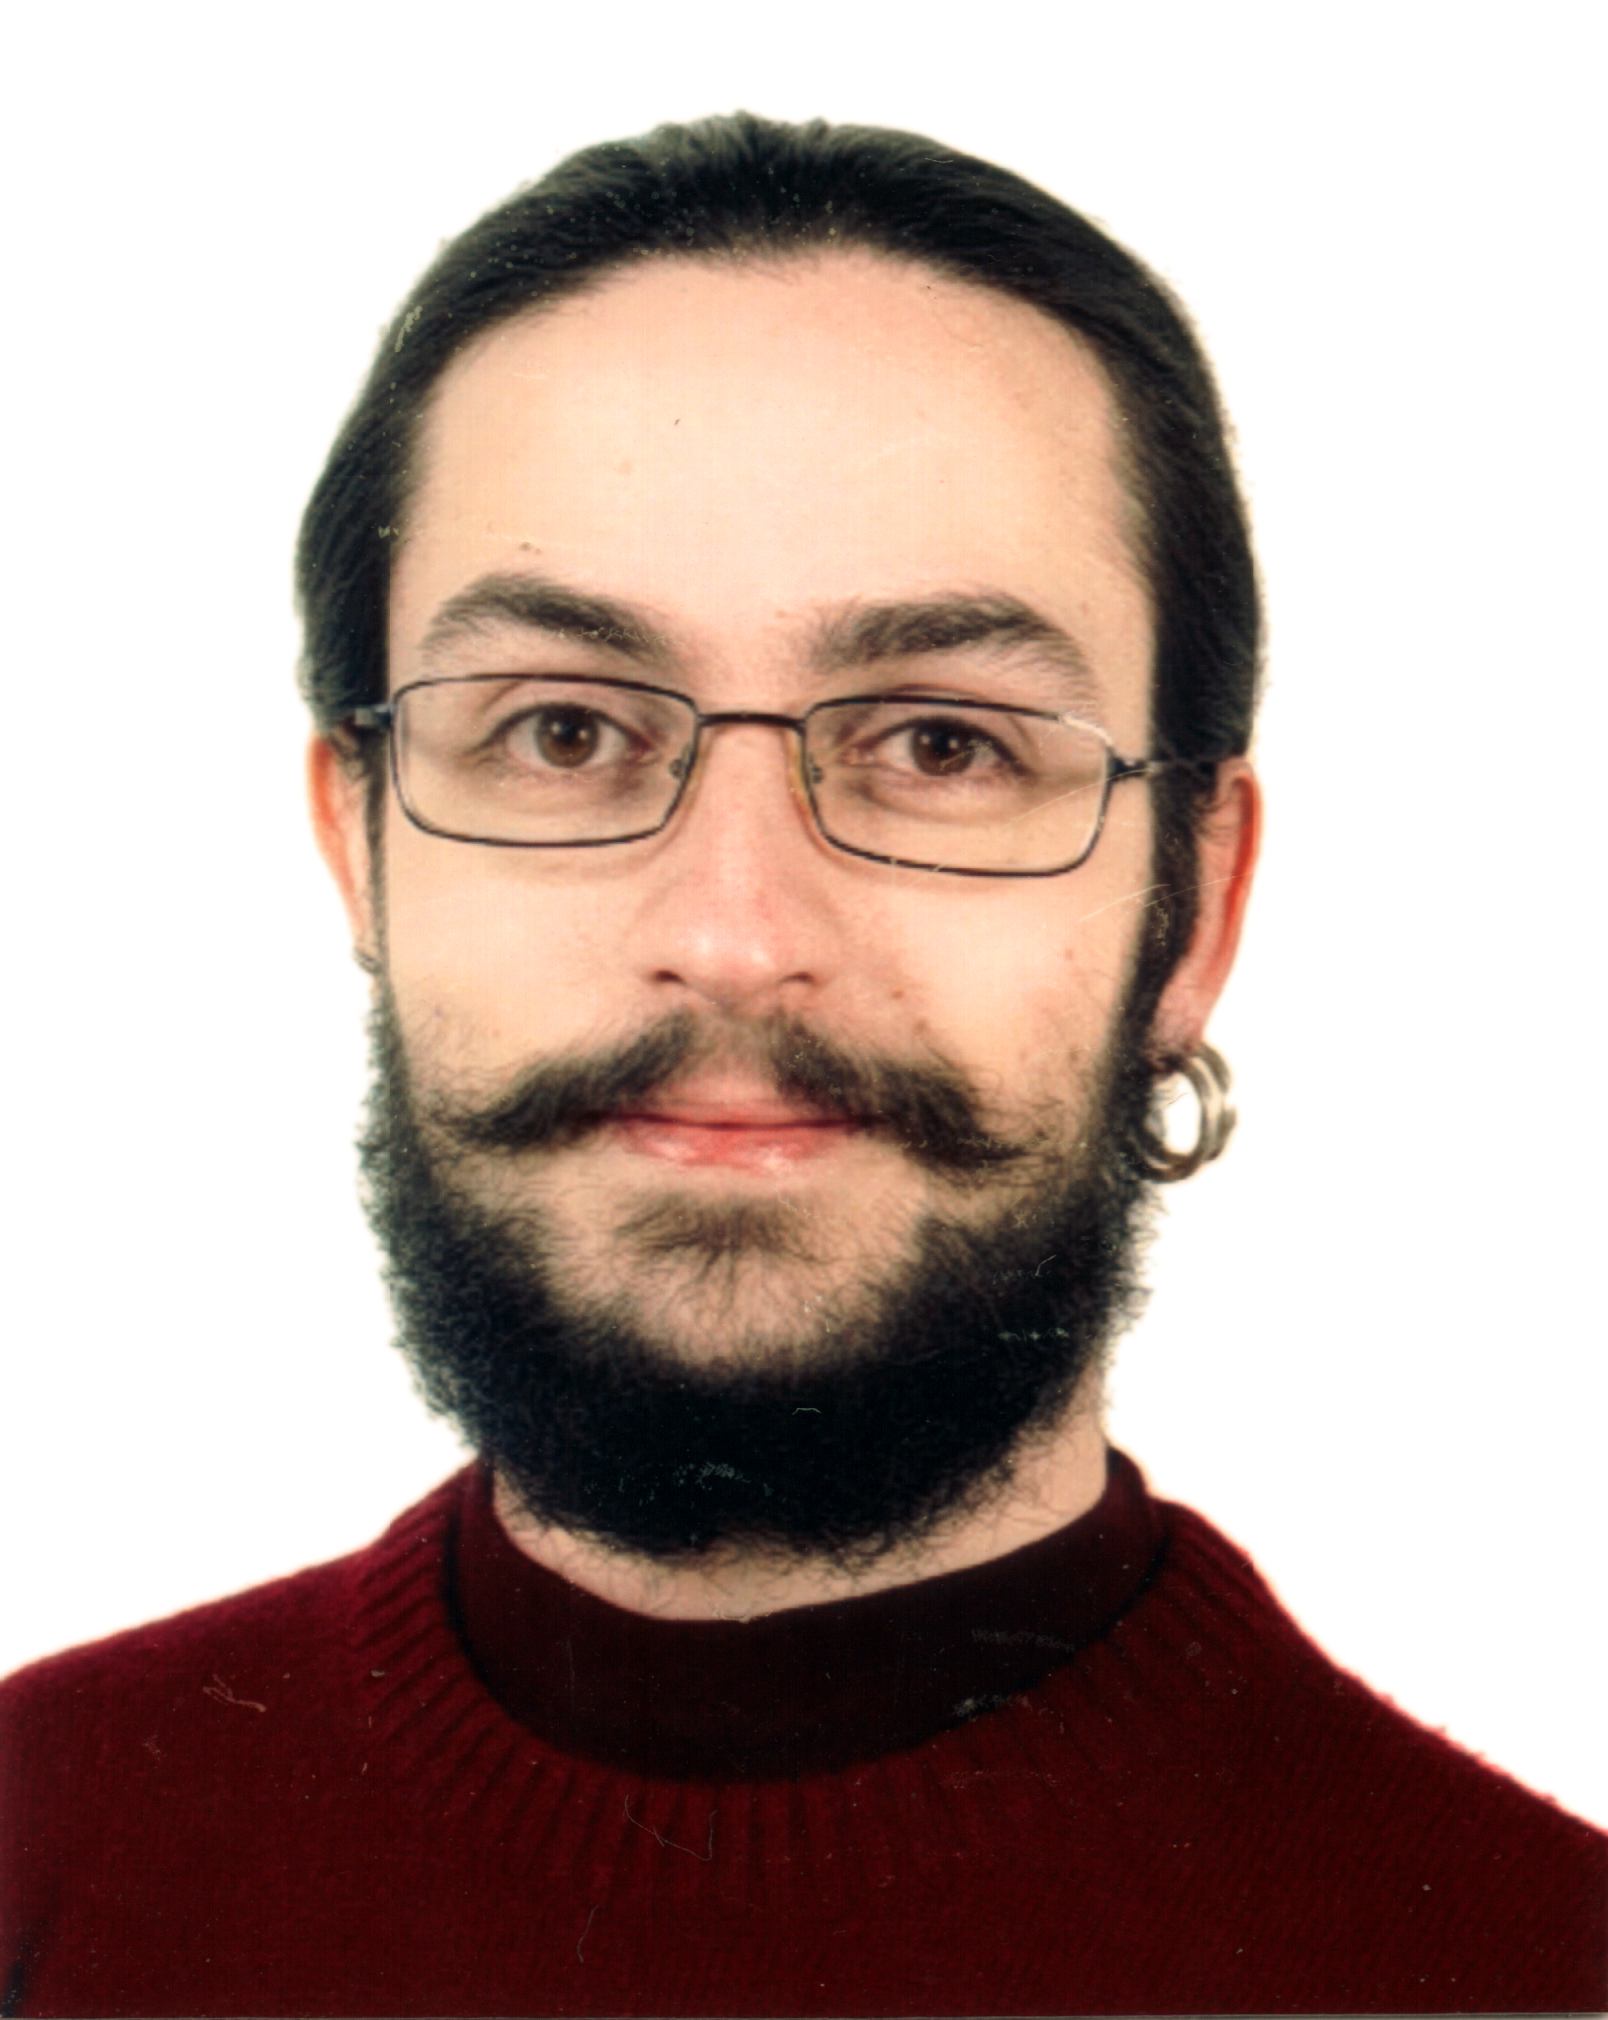
\includegraphics[height=2in]
        {fototessera}};
    \end{scope}
  \end{tikzpicture}}

% \AddToShipoutPictureFG{%
  % \begin{tikzpicture}[remember picture,overlay]
    % \node [
        % draw,
        % text=white,
        % text width=8\q,
        % font=\fontseries{eb}\selectfont,
      % ] at (6\q,32\q)
      % {
      % };
  % \end{tikzpicture}}

\usepackage[
  letterspace=90
]{microtype}

\usepackage{lipsum}

\AddToShipoutPictureFG{%
  \begin{tikzpicture}[remember picture,overlay]
    \node [
        anchor=south,
        % draw,
        inner sep=0,
        text=white,
        text width=8\q,
      ] at (6\q,3\q)
      {
        \SideSection{Contatti}
        \url{paolo.brasolin@gmail.com}
        \hfill\Fa{Envelope}\par\smallskip
        (+39)\ 347\ 6769233
        \hfill\Fa{Phone}\par\smallskip
        \href{https://github.com/paolobrasolin/}{paolobrasolin}
        \hfill\Fa{Github}\par\smallskip
        via Fossalta 38
        \hfill\Fa{Home}\\
        35026 Conselve (PD)\par
        \bigskip
        \SideSection{Lingue}
        \Ranked{Italiano}{5}
        \Ranked{Inglese}{4}
        \Ranked{Francese}{2}
        \bigskip
        \SideSection{Abilità}
        \Ranked{Problem solving}{5}
        \Ranked{Precisione}{4}
        \Ranked{Professionalismo}{3}
        \Ranked{Comunicazione}{3}
        \bigskip
        \SideSection{Competenze}
        \Ranked{\TeX}{5}
        \Ranked{HTML/CSS}{4}
        \Ranked{JavaScript}{3}
        \Ranked{Python}{3}
        \Ranked{Linux}{3}
        \Ranked{Git}{3}
        \Ranked{Ruby}{2}
        \Ranked{Altri linguaggi:
          Haskell, Bash, Perl, C, C++,
          Processing, Mathematica, Lua,
          PHP, SQL, \ldots}{1}
        \bigskip
        \SideSection{Progetti personali}
        \color{white}
        \begin{itemize}
          \item {\scshape koDi}, \TeX\ package for commutative diagrams \emph{done right}
          \item {\tt jekyll-tex}, Ruby gem for HQ static typography on the web
          \item consolidare pratiche TDD a \TeX\ mediante Ruby e Cucumber
        \end{itemize}
        \bigskip
        \SideSection{Interessi}
        Matematica pura.
        Tipografia.
        Grafemica e fonetica.\\
        Musica e fai da te.\par
      };
  \end{tikzpicture}}







\begin{document}

\Section{Profilo}

Sono un programmatore per vocazione e posseggo una solida formazione scientifica.
Cerco un team in cui integrarmi per apprendere le migliori pratiche dello sviluppo
in squadra collaborando alla realizzazione di progetti complessi.
La mia cifra è una grande versatilità coniugata ad una forte propensione
all'apprendimento, oltre che ad una curiosità feroce.

\Section{Esperienza}

\Event
  {Programmatore e document designer}
  {freelancer}
  {2015 -- ora}

Stando in contatto diretto coi clienti ho sperimentato le dinamiche di
negoziazione e determinazione delle specifiche. I miei progetti maggiori
si sono incentrati sull'automazione nella produzione di documenti --
l'intersezione delle mie due principali competenze. Alcuni esempi:

\begin{itemize}[twocol]
  \item webapp (MeteorJS) per gestione di clienti, evasione di ordini,
  compilazione, produzione (\TeX) e consegna di rapporti;
  \item web API (Perl) per la produzione (\TeX) di rapporti PDF compilati
  con form dinamici generati da modelli user-friendly (YAML);
  \item strumenti (Python, \TeX) integrati a sorgenti di dati preesistenti
  (mySQL, CSV) per la produzione di rapporti aziendali;
  \item strumenti per la produzione di business plan parametrici per la
  stampa (\TeX) e dinamici per il web (JS).
\end{itemize}

\Event
  {Programmatore}
  {Ideasmart}
  {2016}

Nella posizione di lead tecnico e sviluppatore fullstack ho esplorato un
concetto di startup gettandone le fondamenta. Gli obbiettivi raggiunti
includono:

\begin{itemize}
  \item scegliere le tecnologie più adeguate ad una realizzazione rapida;
  \item sviluppo del MVP, una app web/Android, col framework MeteorJS;
  \item incapsulamento di interfacce web (ASP.NET) obsolescenti in
  wrapper e scraper (NodeJS, Python) facilmente integrabili nel processo
  di automazione principale.
\end{itemize}

\Event
  {Insegnante}
  {tutor privato}
  {2010 -- ora}

Insegnando materie scientifiche ho potuto rivalutare criticamente la
mia stessa esperienza di studente, lavorando con studenti in prevalenza
universitari.  Mettendo in atto varie tattiche per rendere accessibili
concetti ed astrazioni ho potuto rafforzare le mie doti comunicative.

\Section{Formazione}

% \Event
  % {Master in Security Intelligence}
  % {Istituto Formativo Europeo}
  % {2017 -- ora}

% Questo percorso di Alta Formazione è il giusto complemento alla mia
% esperienza nello sviluppo per potere gestire progetti ad alto profilo
% di sicurezza.

\Event
  {Laurea Magistrale in Fisica Teorica}
  {Università di Padova}
  {2010 -- (2013)}

Frequentata con massimo profitto; interrotta poco prima del conseguimento
in favore di stimoli alternativi all'accademia.
Il percorso mi ha condotto a perfezionare le mia abilità di problem solver e
praticando una strenua ricerca indipendente
trascendendo il curriculum ho guadagnato, oltre ad un'ampia
preparazione matematica, notevoli capacità di astrazione e sintesi.

\Event
  {Laurea in Fisica}
  {Università di Padova}
  {2007 -- 2010}

Conseguita con una tesi sulla Teoria di Stringa.
Il percorso costituisce il solido fondamento della mia formazione scientifica.
Mi ha permesso di alimentare la mia predisposizione naturale al pensiero critico
maturando forti capacità analitiche.

\end{document}
